% !TEX root = ./main.tex
\graphicspath{{figures_RANS_naca0012/}}% Set graphics path location

\subsection{NACA 0012 airfoil at 0$\degr$ angle of attack, Re = 6 million, Ma = 0.15}
In this section, the NACA 0012 airfoil is used to study the accuracy of the SA turbulence model coupled with FR. The NACA 0012 is commonly used as a validation case for all turbulence models and a large database of results are available at the NASA Turbulence Modeling Resource website. A 6,539 element quad/triangle mixed mesh is used with a NACA 0012 airfoil of chord length 1.0 and a farfield boundary 20 chord lengths away. The results are compared with CFL3D and experimental results from Gregory \& O'Reilly, NASA R\&M 3726, Jan 1970.

\begin{figure}
  \begin{subfigmatrix}{2}
    \subfigure[Zoomed view of the mixed element mesh near the NACA 0012 airfoil.]{\includegraphics{NACA0012_Re6mil_mesh.eps}}
    \subfigure[X-momentum contours near the NACA 0012 airfoil]{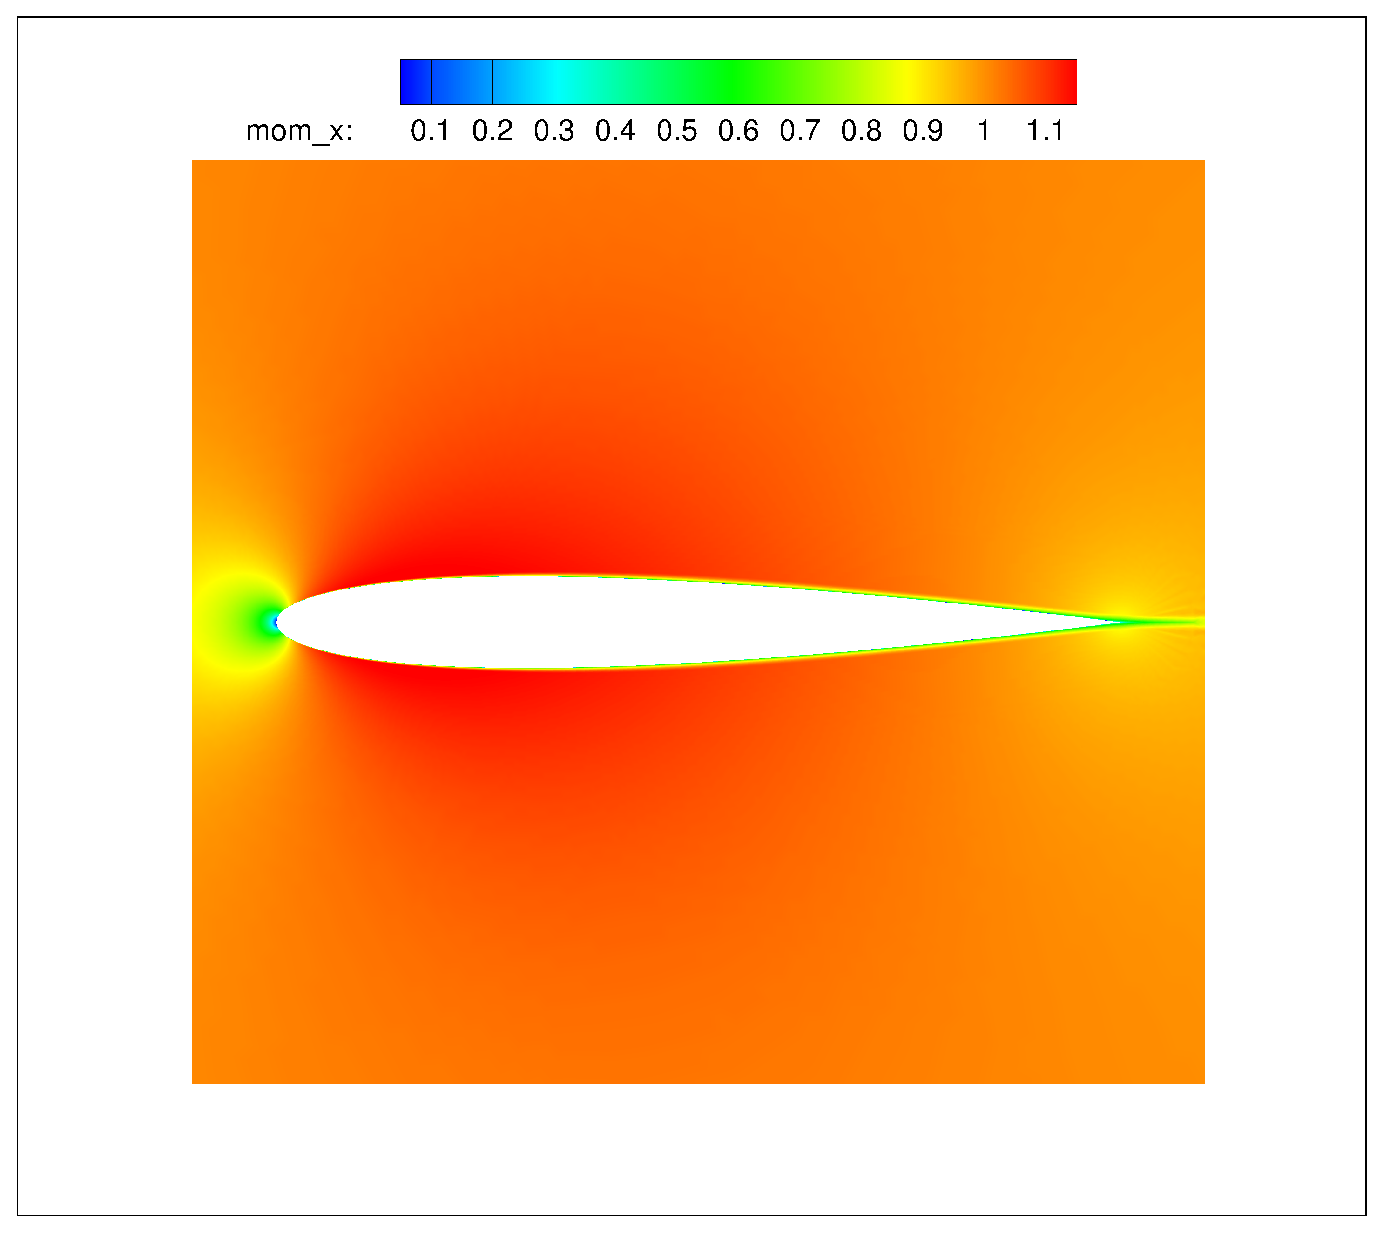
\includegraphics{NACA0012_Re6mil_alp0_momx.eps}}
  \end{subfigmatrix}
  \caption{Turbulent flow past a NACA 0012 airfoil at Re = 6 million, Ma = 0.15, $\alpha = 0^{\circ}$ using FR to recover 4th order accurate DG method and the SA turbulence model.}
  \label{RANS_naca0012}
\end{figure}

\begin{figure}
\centering
  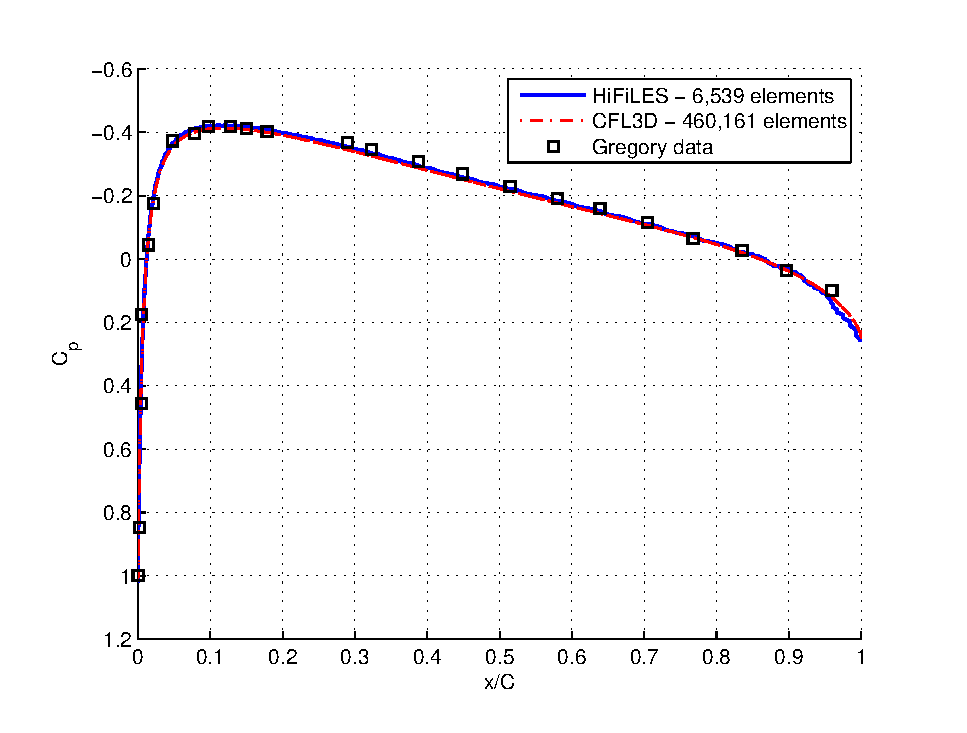
\includegraphics[width=0.48\textwidth]{cp.eps}
  \caption{Pressure coefficient on the NACA 0012 airfoil at Re = 6 million, Ma = 0.15, $\alpha = 0^{\circ}$ using FR to recover 4th order accurate DG method and the SA turbulence model.}
  \label{RANS_naca0012_cp}
\end{figure}

